%%%%%%%% MLSys 2027 submission %%%%%%%%%%%%%%%%%
\documentclass{article}

\usepackage{microtype}
\usepackage{graphicx}
\usepackage{booktabs}
\usepackage{amsmath}
\usepackage{caption}
\usepackage{subcaption}
\usepackage{xcolor}
\usepackage{tikz}
\usepackage{pgfplots}
\pgfplotsset{compat=1.18}
\usetikzlibrary{arrows.meta, positioning, fit, backgrounds, calc, patterns}
\usepackage[section]{placeins}

\usepackage[numbers]{natbib}
\usepackage{hyperref}
\newcommand{\theHalgorithm}{\arabic{algorithm}}

% Blind review copy: do NOT pass [accepted] -- the style file strips author
% info automatically. Switch to \usepackage[accepted]{mlsys2026} and restore
% the Acknowledgments section only for the camera-ready version.
\usepackage{mlsys2026}
% mlsys2026.sty invokes \setcitestyle{authoryear,...} internally; our references are a manual
% thebibliography list with no author-year keys, so re-force numeric mode explicitly rather than
% relying on natbib's own auto-recovery-after-error behavior.
\setcitestyle{numbers,square}

\mlsystitlerunning{Does Metal Performance Primitives Deliver? An MLSys 2027 Submission}

\newcommand{\code}[1]{\texttt{#1}}

\definecolor{seriesFull}{HTML}{2A78D6}
\definecolor{seriesWindowed}{HTML}{EB6834}
\definecolor{seriesAqua}{HTML}{1BAF7A}

\begin{document}

\twocolumn[
\mlsystitle{Does Metal Performance Primitives Deliver? Kernel-, Algorithm-, and
Architecture-Level Optimization for Diffusion Transformer Inference on Apple Silicon}

\begin{mlsysauthorlist}
\mlsysauthor{Anonymous Authors}{}
\end{mlsysauthorlist}

\mlsysaffiliation{}{Anonymous Institution, Anonymous City, Anonymous Region, Anonymous Country}

\mlsyscorrespondingauthor{Anonymous Author}{anonymous@email.com}

\mlsyskeywords{Machine Learning, MLSys, Apple Silicon, Metal, GPU kernels, diffusion models, attention}

\vskip 0.3in

\begin{abstract}
Apple's M5 generation exposed its new per-GPU-core Neural Accelerators through Metal Performance
Primitives (MPP) and its \code{matmul2d} API. We present a falsification-driven empirical study of
whether hand-written \code{matmul2d} kernels outperform PyTorch's native MPS backend
(\code{MPSGraph}) on TRELLIS, an image-to-3D diffusion transformer ported to run natively on Apple
Silicon. Across six operand-type combinations, a precision-relaxation flag, and three successive
attention-kernel designs, hand-written kernels do not reliably beat \code{MPSGraph}: near-parity
single-run results (0.97--1.01$\times$) sit within the $\sim$25\% run-to-run noise we separately
measure by repeated trial at the same latency scale, and only our best flash-attention kernel's
repeatable 1.17$\times$-\emph{slower}-than-native gap is large enough to treat as a real effect.
The paper's most robust systems finding is a repeated-trial ($n{=}20$) comparison against MLX and
\code{llama.cpp}/GGML: MLX's attention kernel is 4.02$\times$ faster than PyTorch's SDPA at the
identical shape, while \code{llama.cpp}'s own hand-tuned kernel is itself \emph{slower} than
PyTorch at the same shape -- evidence the ceiling our kernel work approached is specific to
PyTorch's MPS backend and to MLX's particular kernel design, not a general hardware or non-MPP
effect. This pattern replicates at a substantially different, but still long-sequence, shape
(Llama-2-7B-like), and narrows sharply but does not reverse at a genuinely different model family
and a short-sequence regime (ViT-L/14, $L{=}257$): MLX remains faster there too, but by
$1.18\times$ rather than $4.02\times$, and only after we caught and corrected our own first
measurement, which showed the opposite direction and did not replicate across 8 independent
re-runs -- a real methodological finding in its own right about how much replication
sub-millisecond attention measurements need before trusting their sign. A same-shape check of
PyTorch's own CUDA backend selection on an NVIDIA H200 shows no comparable narrowing or
instability, suggestive (not confirmed) that this is specific to Apple Silicon/MLX rather than a
universal short-sequence property. Motivated
by this modest kernel-level ceiling, we exploit an algorithmic redundancy in TRELLIS's
classifier-free-guidance sampler: a difference-caching fix -- diagnosed against published caching
mechanisms rather than a newly invented one -- delivers a repeatable 1.17--1.30$\times$ speedup,
combined with training-free step reduction (up to 1.98$\times$), both verified across six (image,
seed) combinations. Finally, we replace most self-attention with local windowed attention: a
repeated-trial ($n{=}8$) measurement shows window size, not just how many blocks are windowed,
governs wall-clock speedup, yielding a statistically confirmed 1.12$\times$ full-model speedup once
the right window size is found, with post-distillation quality mixed but modest against a
seed-variance baseline. All code, kernels, and measurement scripts are released for
reproducibility.
\end{abstract}
]

\printAffiliationsAndNotice{}

\section{Introduction}

\begin{figure}[t]
    \centering
    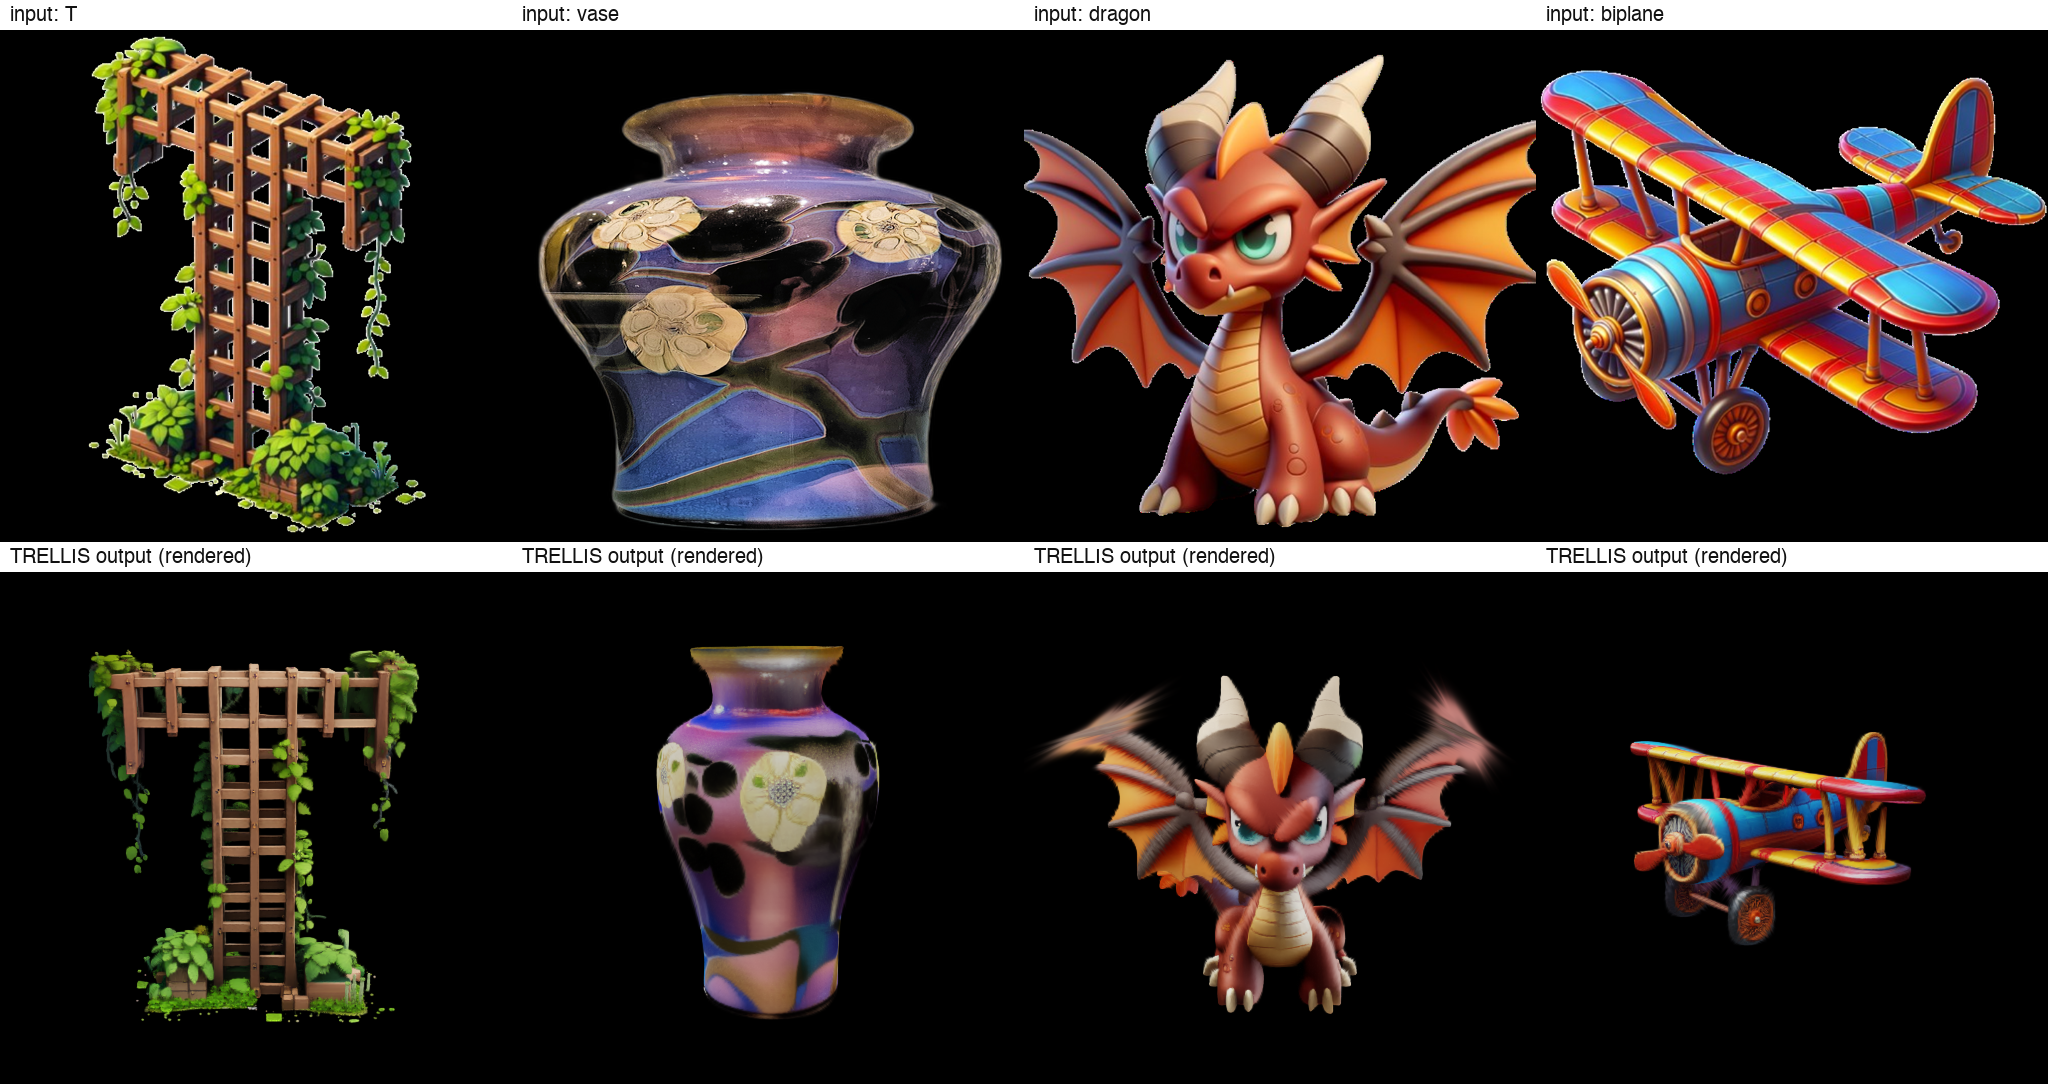
\includegraphics[width=0.95\linewidth]{../figures/fig0_teaser_input_output.png}
    \caption{Example inputs and corresponding TRELLIS-generated 3D outputs (rendered, Gaussian
    splat color channel) from the Apple Silicon port used throughout this study.}
    \label{fig:teaser}
\end{figure}

Apple Silicon GPUs lack dedicated matrix-multiplication ``tensor core'' hardware; matrix
multiplication has historically executed through the same general-purpose ALU pipeline as every
other GPU workload. The M5 generation (announced October 2025) is the first to introduce dedicated
per-GPU-core \emph{Neural Accelerators}, exposed through \emph{Metal Performance Primitives} (MPP),
a Metal~4.1 API centered on \code{matmul2d}. MPP is new enough that, to our knowledge, no
systematic study exists of whether hand-written kernels built on it outperform Apple's existing,
heavily-tuned \code{MPSGraph}-backed path inside a real deployed inference workload, as opposed to
a synthetic microbenchmark.

We use TRELLIS~\cite{trellis2024}, a rectified-flow image-to-3D generation model, as testbed,
porting the full pipeline to run natively via PyTorch's MPS backend, and ask a falsifiable
question: \emph{can hand-written int8-quantized \code{matmul2d} kernels, applied to Linear
projections and attention, measurably speed up real end-to-end inference?} We answer with a chain
of experiments, each testing one hypothesis against direct measurement, escalating in kernel
sophistication only when a simpler design is shown insufficient.

Having found a modest kernel-level ceiling, we turn to an algorithmic question: TRELLIS's
classifier-free-guidance (CFG) sampler recomputes an unconditional prediction every guided step.
Naively caching it causes real, visually-observable drift; we root-cause the failure against
published CFG-caching mechanisms and fix it with a difference-caching scheme specific to
rectified-flow sampling with a guidance interval.

Finally, since attention is $\sim$77\% of forward-pass time (Section~\ref{sec:ffn}) yet
kernel-level attention optimization approaches but does not surpass native latency
(Section~\ref{sec:flash}), we ask whether an architectural change -- not a faster kernel for the
same computation -- can reduce this cost with only a light fine-tune to recover quality. We replace
most self-attention with local windowed attention, retaining full attention periodically for
long-range coherence, and find window size, not merely how many blocks are windowed, determines
whether this helps or hurts wall-clock latency.

\paragraph{Contributions.}
\begin{itemize}
    \item A falsification-driven characterization of \code{matmul2d} across six operand-type
    combinations, a precision-relaxation flag, and three successive attention-kernel designs,
    against real PyTorch MPS baselines on real Apple M5 Max hardware.
    \item A working online-softmax (flash-attention-style) MPP kernel, with a root-caused
    correctness bug and a verified optimization (bookkeeping parallelization) closing a
    $2.9\times$ gap to $1.17\times$.
    \item Real, quantitative framework baselines against MLX and \code{llama.cpp}/GGML: MLX's
    attention kernel is $4.02\times$ faster than PyTorch's native SDPA at the identical shape,
    while \code{llama.cpp}'s independent hand-tuned kernel is \emph{slower} than PyTorch --
    evidence the ceiling we approached is specific to PyTorch's MPS backend, and to MLX's design
    rather than any non-MPP approach. Confirmed at a substantially different (Llama-2-7B-like)
    shape profile; narrows sharply but does not reverse at a genuinely different model family and
    a short-sequence shape (ViT-L/14, $4.02\times \to 1.18\times$), after catching and correcting
    our own first measurement there, which showed the opposite direction and failed to replicate
    across 8 independent re-runs. A cross-hardware (NVIDIA H200) check finds no comparable
    narrowing or instability, suggestive this is specific to Apple Silicon/MLX.
    \item A difference-based CFG-caching scheme for TRELLIS's rectified-flow guidance-interval
    sampler, with a documented failure mode, root cause, and fix grounded in published mechanisms
    (FasterCache, AB-Cache), verified quantitatively and qualitatively across six (image, seed)
    combinations.
    \item A combined, training-free speedup recipe (step reduction + CFG difference caching)
    delivering reproducible wall-clock improvements without retraining.
    \item An architecture-level bypass measurement isolating self-attention (29.3\% of
    forward-pass time) from cross-attention (12.5\%), and an interleaved full/windowed
    self-attention design whose real speedup depends critically on window size -- a smaller
    window that is naively cheaper in FLOPs is measurably \emph{slower} in wall-clock terms, while
    a larger window yields a statistically confirmed 1.12$\times$ full-model speedup.
\end{itemize}

\section{Background and Related Work}
\label{sec:background}

\textbf{TRELLIS}~\cite{trellis2024} generates 3D assets from a single image via two cascaded
rectified-flow diffusion transformers: a sparse-structure model (555.5M parameters, 24 blocks)
sampling coarse voxel occupancy, and a structured-latent model (600.4M parameters) sampling
per-voxel latent features, decoded to mesh, Gaussian-splat, or radiance-field representations. Both
use \code{FlowEulerGuidanceIntervalSampler} (a first-order Euler integrator with CFG restricted to
$t \in [0.5,1.0]$ of 25 steps, guidance strength $s{=}5.0$) and load natively in \code{float16}.

\textbf{Metal Performance Primitives.} \code{matmul2d} performs $C=AB(+C)$ over tiled
thread-group-cooperative execution scopes, supporting $\sim$46 documented operand-type
combinations (\code{half}, \code{int8\_t}/\code{uint8\_t}, \code{float}, \code{bfloat}, 4-bit
packed), including native mixed-precision \code{half}$\times$\code{int8\_t}$\to$\code{float}. A
\code{relaxed\_precision} flag is documented to trade accuracy for speed.
\code{cooperative\_tensor} chains one \code{matmul2d} call's output directly into another without
a device-memory round trip, but (Section~\ref{sec:coop-tensor}) is restricted to single-simdgroup
scopes.

\textbf{Related work.} FlashAttention~\cite{flashattention} established that attention's real cost
is dominated by device-memory traffic, not FLOPs -- the same hypothesis motivates our
online-softmax kernel progression (Section~\ref{sec:flash}), on Apple's unified-memory/MPP tiling
model rather than CUDA's. LLM.int8()~\cite{llmint8} showed int8 weight-and-activation quantization
can preserve accuracy via outlier isolation; our operand sweep instead holds accuracy fixed and
asks whether \emph{any} MPP low-precision combination reaches native latency on this hardware. The
Swin Transformer~\cite{swin} introduced shifted local-window attention for vision transformers; we
reuse its shift pattern but ask whether it helps a \emph{diffusion denoiser's} wall-clock latency
once real partition/gather overhead is accounted for -- which Section~\ref{sec:window-size} shows
is not guaranteed by FLOP reduction alone. Our CFG difference-caching
(Section~\ref{sec:cfg-caching}) is grounded in FasterCache~\cite{fastercache} and
AB-Cache~\cite{abcache}'s published mechanisms.

\section{Methodology}

Every kernel change passed through four stages: (1) \emph{synthetic correctness} -- varied and
non-tile-aligned shapes, checked against the module's PyTorch fallback and a CPU \code{float32}
reference; (2) \emph{real-model finite-output check} -- the full pretrained model with real image
conditioning across multiple trials, necessary because one correctness bug
(Section~\ref{sec:ffn}) passed every synthetic check yet produced \code{NaN} only under real
weights; (3) \emph{isolated microbenchmark} at real production shapes; (4) \emph{full real-model
benchmark}, the only number treated as reportable, since isolated and real-model speed are shown
(Section~\ref{sec:ffn}) to diverge substantially.

All kernel-, algorithmic-, and architecture-level \emph{wall-clock} measurements ran on a single
Apple M5 Max, macOS~26.4.1, Metal SDK~26.5. Framework baselines used MLX v0.31.2 and a
\code{llama.cpp}/GGML build (\code{GGML\_METAL=ON}) on the same machine, via a standalone harness
against \code{ggml.h}/\code{ggml-backend.h} directly. Two results ran on a separate NVIDIA
H200/CUDA machine instead: the architecture-level \emph{distillation training and quality
validation}, purely to make fine-tuning practical (the fine-tuned weights are hardware-independent,
but the quality numbers were not independently re-verified on the Apple Silicon target hardware);
and the ViT-L/14 cross-hardware CUDA-backend-selection check
(Section~\ref{sec:framework-baselines}), run deliberately on different hardware since its entire
purpose is checking whether a short-sequence effect generalizes beyond Apple Silicon/MPS.

\section{Kernel-Level Results}
\label{sec:ffn}

\subsection{FFN: an architectural ceiling}
We quantized the FFN block
(\code{fc1}$\to$\code{GELU}$\to$\code{fc2}) to int8 via \code{matmul2d}, fused through
\code{torch.compile}. Bypass measurement on the sparse-structure flow model (the denoiser used for
all kernel-level measurements in this section) showed the FFN is only $\sim$11\% of forward time
despite 36.3\% of parameters -- a $\sim$1.12$\times$ ceiling regardless of kernel quality. Measured
result: 1.11$\times$ \emph{slower}, motivating a shift to attention, which the same method showed
is $\sim$77\% of forward time on this same model. An isolated-vs-real-model discrepancy (1.35 vs.\ 2.50ms/block) was
traced to a benchmark-shape bug, not a cache effect; sweeping working-set size at the correct shape
produced a flat 2.68--2.69ms/call, refuting the cache hypothesis.

\subsection{Quantized attention}
Applying the same pattern to \code{to\_qkv}/\code{to\_q}+\code{to\_kv}/
\code{to\_out} required fixing a real bug (\code{matmul2d}'s custom op always returns
\code{float32}, silently crashing a native \code{float16} \code{nn.Linear} downstream). After the
fix, self-attention's quantized Linears measured \emph{at} native (0.972$\times$), cross-attention's
three separate Linears remained slower (1.189$\times$); full-model: 0.98$\times$. These are
single-run measurements; Section~\ref{sec:framework-baselines}'s repeated-trial baseline shows
$\sim$25\% run-to-run noise at this same latency scale, so 0.97--1.01$\times$-class results
throughout this section should be read as near-parity, not as confirmed wins or losses -- only the
flash-attention kernel's 1.17$\times$ gap (Section~\ref{sec:flash}) is large enough relative to
that noise floor to treat as a real effect.

\subsection{Operand-type sweep}
We swept six of MPP's $\sim$46 documented combinations at the real
\code{to\_qkv} shape (Figure~\ref{fig:combos}). Every combination with a \code{half}/\code{bfloat}
operand clustered $\sim$1.9$\times$ slower than native \code{float16} \code{nn.Linear},
\emph{regardless of the other operand's type} -- ruling out int8 specifically as the bottleneck.
Only full \code{int8\_t}$\times$\code{int8\_t}$\to$\code{int32} reached parity (1.01$\times$), at a
real accuracy cost (median relative error 0.0111 vs.\ 0.0078). The \code{relaxed\_precision} flag
was a clean null: byte-identical output, 1.003$\times$ speed.

\begin{figure}[t]
    \centering
    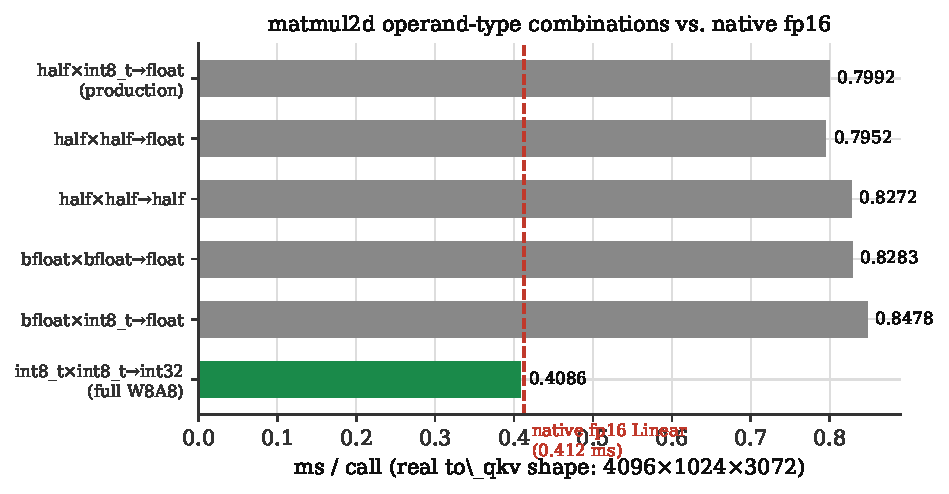
\includegraphics[width=0.95\columnwidth]{../figures/fig1_matmul2d_combos.pdf}
    \caption{\code{matmul2d} speed across six operand-type combinations vs.\ native \code{float16}
    \code{nn.Linear}, at the real \code{to\_qkv} shape. Only full int8 reaches parity; every
    combination with a narrow floating-point operand clusters near $1.9\times$ slower.}
    \label{fig:combos}
\end{figure}

\subsection{Dispatch batching: a falsified hypothesis}
A naive per-head loop measured
$2.8\times$ slower than \code{torch.bmm}, attributed to 16 separate dispatches. Batching all heads
into one \code{dispatchThreads} call produced almost no improvement (1.016$\times$ vs.\ the loop),
falsifying the dispatch-count hypothesis: both remained $\sim$3$\times$ slower than native SDPA.

\subsection{Online-softmax flash-attention}
\label{sec:flash}
The leading remaining hypothesis -- that materializing the full $L\times L$ score matrix in device
memory dominates cost -- led to an online-softmax kernel keeping running statistics in on-chip
memory. A tail-block boundary bug (\code{matmul2d}'s edge-checking left stale threadgroup memory
in invalid tile columns) was fixed by explicit zeroing. The corrected kernel measured 8.41ms
($1.68\times$ slower than native, $1.8\times$ faster than the non-flash batched version). We then
parallelized the bookkeeping (one thread per row $\to$ two lanes via \code{simd\_shuffle\_xor}),
reducing latency to 5.81ms -- only $1.17\times$ slower, the closest of every design tested
(Figure~\ref{fig:progression}). \code{KVBLOCK}$=$64 is infeasible (threadgroup memory budget);
\code{KVBLOCK}$=$16 regressed to 7.97ms; \code{KVBLOCK}$=$32 remains best.

\begin{figure}[t]
    \centering
    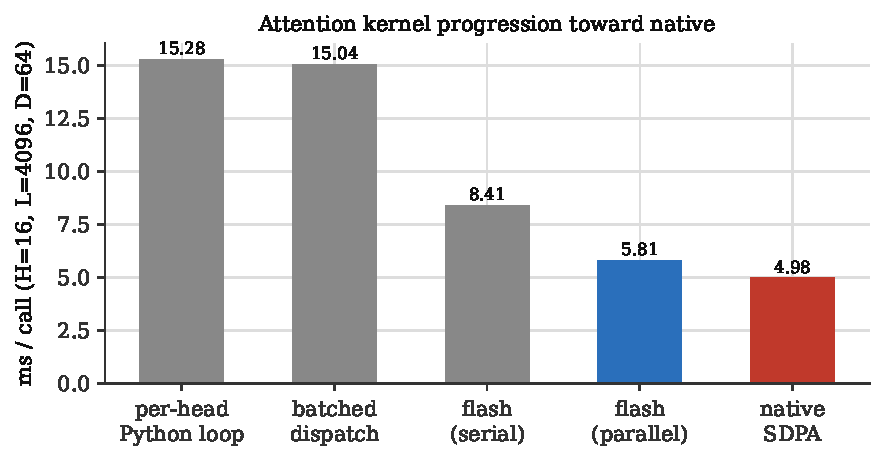
\includegraphics[width=0.95\columnwidth]{../figures/fig2_kernel_progression.pdf}
    \caption{Attention-kernel latency across five successive designs, real self-attention shape
    ($H{=}16, L{=}4096, D{=}64$). Parallelizing online-softmax bookkeeping (blue) closed most of
    the gap to native SDPA (red).}
    \label{fig:progression}
\end{figure}

\subsection{\code{cooperative\_tensor}: a hard architectural constraint}
\label{sec:coop-tensor}
Reading \code{MPPTensorOpsMatMul2dImpl.h} directly revealed a hard \code{static\_assert} requiring
single-simdgroup scope for chaining-input functions; our kernel's tiling uses
\code{execution\_simdgroups<4>}, so a redesign would very likely require smaller tiles and more
dispatches -- the same failure mode already observed to regress performance in tile-size tuning. We
treat this mechanism as closed given 1.17$\times$ already represents the closest approach found.

\subsection{Real framework baselines: MLX and \code{llama.cpp}}
\label{sec:framework-baselines}
This is the paper's most robust systems finding: unlike the single-run kernel numbers above, every
result in this subsection is a repeated-trial ($n{=}20$) measurement with a reported confidence
interval. Reading MLX's~\cite{mlx} shipped attention kernel (\code{sdpa\_vector.h}) shows it uses
manual scalar dot products with \code{simd\_sum}, not \code{simdgroup\_matrix}/MPP. We upgrade this
to a direct, quantitative comparison: real MLX v0.31.2 and a \code{llama.cpp}/GGML~\cite{ggml}
build, run back-to-back against PyTorch MPS on the same machine, at this paper's reference shapes
(Table~\ref{tab:frameworks}, $n{=}20$ trials per configuration). MLX's default attention call uses
no mask, matching PyTorch's default (\code{is\_causal=False}) -- confirmed before trusting the
comparison, since a masking difference between frameworks would invalidate it.

\begin{table}[t]
    \centering
    \caption{Framework comparison at this paper's reference shapes, $n{=}20$ trials, mean
    $\pm$ 95\% CI ($1.96\cdot\text{s.d.}/\sqrt{n}$, the same convention as
    Table~\ref{tab:window-sweep}). The Linear row's raw sample std.\ dev.\ is 0.178ms on a
    0.698ms PyTorch mean ($\sim$25\% relative std.\ dev.) -- this raw run-to-run variability,
    not the tighter CI shown below, is the noise-floor baseline Section~\ref{sec:ffn}'s
    single-run near-1.0$\times$ kernel numbers are read against.}
    \label{tab:frameworks}
    \resizebox{\columnwidth}{!}{
    \begin{tabular}{@{}lrrr@{}}
        \toprule
        Operation & PyTorch MPS & MLX & \code{llama.cpp} \\
        \midrule
        Linear (\code{to\_qkv}) & 0.698$\pm$0.078 & 0.717$\pm$0.088 & \textbf{0.669$\pm$0.024} \\
        Self-attn.\ SDPA & 5.465$\pm$0.089 & \textbf{1.361$\pm$0.037} & 7.166$\pm$0.059 \\
        \bottomrule
    \end{tabular}}
\end{table}

For matmul, all three frameworks cluster near parity. For attention, MLX is $4.02\times$ faster
than PyTorch's native SDPA at the identical shape, while \code{llama.cpp}'s own hand-tuned,
production-grade kernel is \emph{itself slower} than PyTorch (1.31$\times$). A second independent,
actively-optimized implementation does not replicate MLX's advantage, so the $\sim$1.17$\times$
ceiling our kernel reached (Section~\ref{sec:flash}) reflects PyTorch's MPS backend specifically,
not this hardware's achievable ceiling -- and is not simply a property of avoiding MPP-style tiling
in general, since \code{llama.cpp} also avoids it and does not replicate MLX's result. Re-running
the identical comparison at a substantially different, Llama-2-7B-like shape (hidden 4096, 32
heads, $D{=}128$, $L{=}2048$) replicates the pattern: matmul near parity, MLX $3.24\times$ faster at
attention, \code{llama.cpp} $1.17\times$ slower -- evidence this is not an artifact of TRELLIS's
particular shapes (full table in Appendix~\ref{app:generalization-shape}).

\textbf{The pattern narrows sharply at a short-sequence shape, and one measurement here needed
correction.} Both shapes tested so far share one property: long sequences ($L{=}4096$ and
$L{=}2048$). We test a third, genuinely different model family at a short-sequence shape:
ViT-L/14 (CLIP's vision encoder), whose real published configuration (hidden 1024, 16 heads,
$D{=}64$, $L{=}257$ -- 256 image patches plus one CLS token) shares TRELLIS's own channel/head
dimensions but differs by $16\times$ in sequence length (Table~\ref{tab:vit}).

Our first $n{=}20$ measurement at this shape showed PyTorch \emph{faster} than MLX at
self-attention -- an apparent reversal of the long-sequence pattern. Applying this paper's own
verification discipline (Section~\ref{sec:ffn}: never trust a single measurement without a
replication check) before reporting it as a finding, we re-ran the identical script independently
8 more times. The direction did not replicate: MLX was faster in all 8 of 8 follow-up runs, by a
mean ratio of $1.18\times$ (range $1.03$--$2.53\times$ across runs). We treat the original
measurement as a noise artifact, not a real effect, and report the replicated result instead.
Table~\ref{tab:vit} shows one representative run together with the across-run aggregate. At the
Linear shape, the direction is more consistent across repeats: MLX faster by $1.86\times$
(mean of 3 independent full-script runs, range $1.66$--$2.04\times$) -- unlike
Table~\ref{tab:frameworks}'s near-parity matmul result at TRELLIS's own shape, MLX pulls ahead on
matmul at this smaller shape too.

\begin{table}[t]
    \centering
    \caption{Framework comparison at a genuinely different model family and regime: ViT-L/14
    (CLIP), hidden 1024, 16 heads, $D{=}64$, $L{=}257$ (real published config), Apple M5 Max. One
    representative $n{=}20$ run (mean $\pm$ 95\% CI) alongside the across-run aggregate that
    established the replicated direction (mean of independent run-means $\pm$ std.\ dev.\ across
    runs; SDPA: 8 runs, Linear: 3 runs).}
    \label{tab:vit}
    \resizebox{\columnwidth}{!}{
    \begin{tabular}{@{}lrrr@{}}
        \toprule
        Operation & PyTorch MPS (1 run) & MLX (1 run) & Ratio (across-run mean) \\
        \midrule
        Linear (QKV proj.) & 0.479$\pm$0.078 & \textbf{0.289$\pm$0.071} & \textbf{1.86$\times$} \\
        Self-attn.\ SDPA & 0.197$\pm$0.008 & \textbf{0.172$\pm$0.008} & \textbf{1.18$\times$} \\
        \bottomrule
    \end{tabular}}
\end{table}

MLX remains the faster framework at this shape for both operations -- the long-sequence pattern
narrows substantially ($4.02\times \to 1.18\times$ for self-attention) rather than reversing, and
is markedly noisier here: PyTorch's own self-attention latency at this shape showed run-to-run
coefficients of variation as high as 49\% in a large-sample ($n{=}100$) check, roughly double
Table~\ref{tab:frameworks}'s own established $\sim$25\% noise floor and the highest instability we
observed anywhere in this paper. This -- not a direction reversal -- is what actually distinguishes
short from long sequences here: the framework gap shrinks, and the underlying measurement itself
becomes markedly less stable, to the point that a single $n{=}20$ sample (our own first attempt)
produced the wrong sign entirely. We surface this as a methodological finding in its own right:
sub-millisecond attention operations on this hardware need either a much larger $n$ or independent
replication across separate runs before a directional claim is trustworthy, a bar this paper's
other framework-comparison results (Table~\ref{tab:frameworks}, millisecond-scale) comfortably
clear without needing it.

We also checked PyTorch's own CUDA SDPA backend selection at the identical ViT-L/14 shape on an
NVIDIA H200, to see whether short sequences generally erode a specialized kernel's advantage over
a naive default (MLX does not run on CUDA, so this is a same-shape, same-op, different-hardware
comparison of backend-selection behavior, not a literal MLX rerun). The specialized backends
(\code{FLASH\_ATTENTION}: 0.0242ms; \code{EFFICIENT\_ATTENTION}: 0.0269ms) still clearly beat the
naive reference (\code{MATH}: 0.0513ms) by $\sim$1.9--2.1$\times$ at this same short sequence
length, with no comparable instability to what we observed on MPS. (A fourth backend,
\code{CUDNN\_ATTENTION}, was also attempted but failed outright with no available kernel for this
shape/dtype combination on this PyTorch/cuDNN build -- reported for completeness, not omitted by
choice. These H200 numbers are $\sim$9--17$\times$ faster in absolute terms than the M5 Max,
unsurprising for a data-center GPU at this tiny problem size, and not the point of the
comparison.) So CUDA's specialized-vs-naive backend gap does not narrow or destabilize at this
short sequence length the way the MPS-vs-MLX framework gap does -- suggestive that whatever
narrows MLX's advantage at short sequences on Apple Silicon is not a universal property of short
sequences, though with only one cross-hardware data point we state this as a hypothesis, not a
confirmed mechanism.

\section{Algorithmic-Level Results}

\subsection{Step-count reduction}
TRELLIS's rectified-flow formulation should tolerate fewer sampling
steps without a higher-order solver. Reducing from 25 to 20/15/10/8 steps
(Figure~\ref{fig:stepcount}) gave 1.16--1.92$\times$ speedups; voxel-IoU degradation (0.95--0.81)
diverged sharply from visual/mesh signals -- rendered output stayed visually consistent at every
step count, and mesh vertex/face counts stayed in a narrow band (298K--317K), indicating IoU
over-penalizes benign boundary-voxel discretization noise.

\begin{figure}[t]
    \centering
    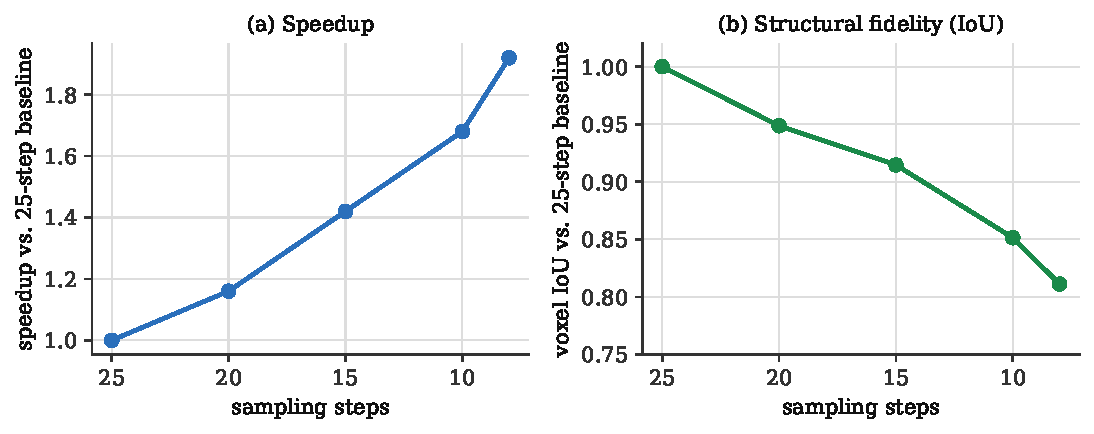
\includegraphics[width=0.95\columnwidth]{../figures/fig3_step_count_tradeoff.pdf}
    \caption{Speedup and structural fidelity (voxel IoU vs.\ 25-step baseline) as sampling steps
    reduce. IoU degrades faster than visual quality.}
    \label{fig:stepcount}
\end{figure}

\begin{figure}[t]
    \centering
    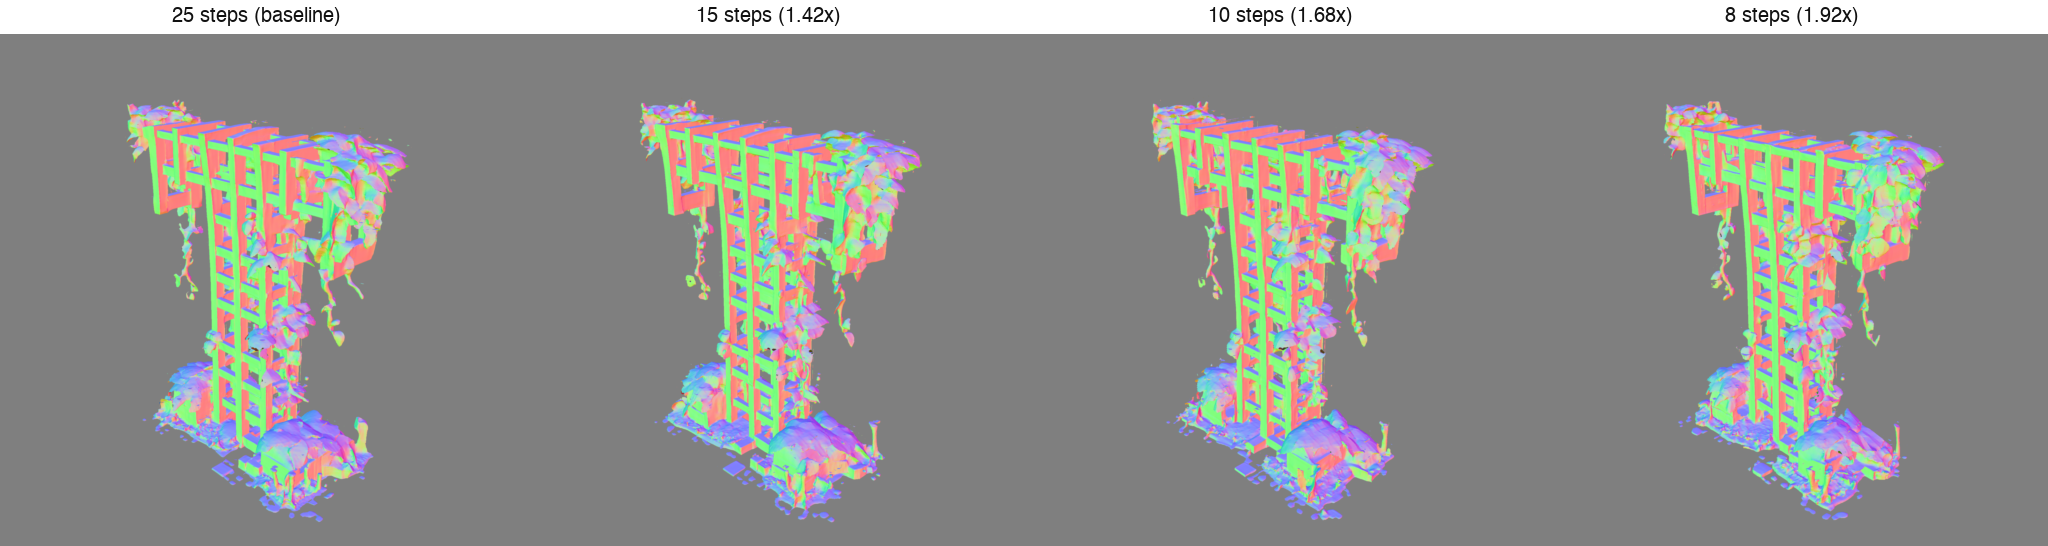
\includegraphics[width=0.95\columnwidth]{../figures/fig5a_step_count_qualitative.png}
    \caption{Rendered surface-normal previews at each tested step count. No visible quality
    collapse down to 8 steps, despite voxel IoU dropping to 0.81 at that setting.}
    \label{fig:step_qual}
\end{figure}

\subsection{CFG-caching: failure, root cause, fix}
\label{sec:cfg-caching}
TRELLIS's CFG sampler calls the denoiser twice per guided step, combining
$\hat{v}=(1{+}s)v_{\mathrm{cond}}-s\,v_{\mathrm{uncond}}$. Caching $v_{\mathrm{uncond}}$ verbatim
for $N$ steps produced real drift that \emph{grew} with interval: mesh vertex count rose
monotonically from 313{,}772 (no caching) to 394{,}129 (interval 4), with visible extraneous
geometry. Tracing this against FasterCache~\cite{fastercache} and AB-Cache~\cite{abcache}'s actual
mechanisms -- neither freezes a raw branch; both cache \emph{differences}, and AB-Cache documents
that larger guidance scale amplifies stale-difference error, directly relevant given TRELLIS's
$s{=}5.0$ -- we instead cache $d=v_{\mathrm{cond}}-v_{\mathrm{uncond}}$ and derive
$\hat{v}_{\mathrm{uncond}}=v_{\mathrm{cond}}^{\mathrm{fresh}}-d$ at no extra model-call cost
(Table~\ref{tab:cfg}). Our contribution here is the diagnosis, not a new caching mechanism: the
difference-caching idea itself is FasterCache/AB-Cache's; what is new is root-causing naive
caching's failure against this specific sampler family (rectified-flow with a guidance-interval,
$s{=}5.0$) and showing the published mechanism transfers to it without modification.

\begin{table}[t]
    \centering
    \caption{CFG-caching: naive freezing vs.\ difference-caching (ours).}
    \label{tab:cfg}
    \resizebox{\columnwidth}{!}{
    \begin{tabular}{@{}lrrrr@{}}
        \toprule
        Method & Interval & Speedup & Vertices & IoU \\
        \midrule
        Baseline & 1 & 1.00$\times$ & 313{,}772 & 1.0000 \\
        Naive & 2 & 1.13$\times$ & 336{,}719 & 0.8794 \\
        Naive & 4 & 1.12$\times$ & 394{,}129 & 0.6787 \\
        Ours (diff.) & 2 & 1.17$\times$ & 316{,}150 & 0.8994 \\
        Ours (diff.) & 4 & \textbf{1.29$\times$} & 309{,}281 & 0.7913 \\
        \bottomrule
    \end{tabular}}
\end{table}

\begin{figure}[t]
    \centering
    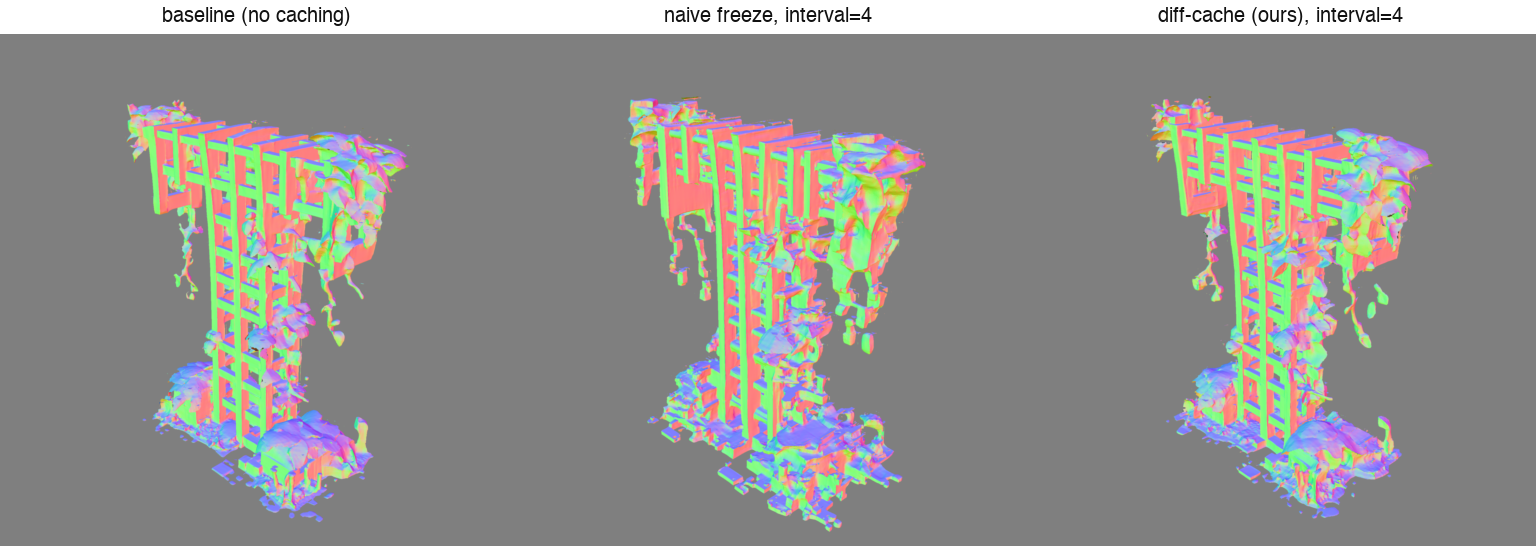
\includegraphics[width=0.95\columnwidth]{../figures/fig5b_cfg_caching_qualitative.png}
    \caption{Rendered comparison at interval 4: naive freezing introduces visible extraneous
    geometry; difference-caching (ours) does not.}
    \label{fig:cfg_qual}
\end{figure}

\subsection{Generalization}
Both techniques were re-verified at their most aggressive setting (8
steps; interval 4) against three additional images (inorganic, organic, mechanical) at two seeds
each. Step reduction averaged $1.98\times$ at 0.879 IoU; difference-caching averaged $1.22\times$ at
0.815 IoU. Both held on every combination, with no repeat of naive caching's drift signature (full
per-image table in Appendix~\ref{app:generalization-images}).

\section{Architecture-Level Results}
\label{sec:architecture}

Motivated by attention's $\sim$77\% time-share (Section~\ref{sec:ffn}) yet kernel-level attention
optimization not surpassing native latency (Section~\ref{sec:flash}), we ask whether an
architectural change -- not a faster kernel -- can reduce this cost with only a light fine-tune.

\subsection{Self- vs.\ cross-attention}
A bypass measurement on the structured-latent denoiser found
self-attention responsible for 29.3\% of forward-pass time (91.15ms of 310.60ms) vs.\
cross-attention's 12.5\% (38.75ms) -- individually-bypassed contributions sum within 0.01ms of the
joint bypass, confirming no interaction effect. This combined share (41.8\%) is lower than
Section~\ref{sec:ffn}'s $\sim$77\%: the two numbers describe two different models in the pipeline
(sparse-structure vs.\ structured-latent), not the same measurement disagreeing with itself.
Self-attention, unlike cross-attention (restricted to full attention by construction), is free to
be replaced with a cheaper local mechanism.

\subsection{Interleaved full/windowed attention}
We replace most self-attention with local windowed
attention (Swin-style shift pattern, already used but unbenchmarked in this codebase's own VAE
decoders), retaining full attention every $K$ blocks. Since attention mode is a pure forward-time
flag, this is a direct, in-place modification -- a full-attention checkpoint's weights remain valid
immediately after the swap, no reinitialization required.

\begin{figure}[t]
    \centering
    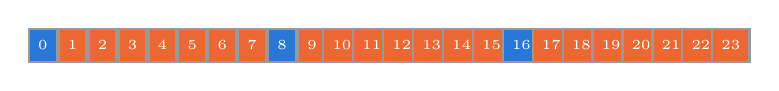
\begin{tikzpicture}[
        blk/.style={rectangle, draw=black!40, minimum width=0.34cm, minimum height=0.42cm, font=\fontsize{4}{4.5}\selectfont, thick},
        fullblk/.style={blk, fill=seriesFull, text=white},
        winblk/.style={blk, fill=seriesWindowed, text=white},
    ]
        \foreach \i in {0,...,23} {
            \pgfmathtruncatemacro{\iscol}{mod(\i,8)==0 ? 1 : 0}
            \ifnum\iscol=1
                \node[fullblk] (b\i) at (\i*0.38, 0) {\i};
            \else
                \node[winblk] (b\i) at (\i*0.38, 0) {\i};
            \fi
        }
    \end{tikzpicture}
    \caption{24-block self-attention assignment at $K{=}8$: full attention every 8th block (blue),
    local windowed attention elsewhere (orange). Full connectivity vs.\ windowed-connectivity
    schematic in Appendix~\ref{app:arch-diagram}.}
    \label{fig:block-strip}
\end{figure}

\subsection{Window size, not just $K$, determines the speedup}
\label{sec:window-size}
At the window size already trusted elsewhere in this codebase ($W{=}8$), even the most aggressive
setting ($K{=}24$) reached only $\sim$1.05--1.08$\times$. Isolating windowed attention itself
revealed why: at $W{=}8$ it is $2.1\times$ \emph{slower} than full attention in isolation
(partition/gather overhead dominates); only $W{=}16$ is genuinely faster in isolation
($1.47\times$). We ruled out a warm-up confound (reverse-order re-run replicated the trend) and
re-benchmarked $W{=}16$/$W{=}32$ with $n{=}8$ trials and 95\% CIs (Table~\ref{tab:window-sweep},
Figure~\ref{fig:window-sweep-plot}).

\begin{table}[t]
    \centering
    \caption{Full-model speedup vs.\ baseline, by $W$ and $K$, $n{=}8$ trials, 95\% CI.}
    \label{tab:window-sweep}
    \resizebox{\columnwidth}{!}{
    \begin{tabular}{@{}lrrr@{}}
        \toprule
        $K$ & $W{=}8$ & $W{=}16$ & $W{=}32$ \\
        \midrule
        1 (baseline) & 1.000$\times$ & 1.000$\times$ & 1.000$\times$ \\
        2  & 1.025$\pm$0.046 & 1.058$\pm$0.012 & 1.064$\pm$0.006 \\
        3  & 1.069$\pm$0.043 & 1.080$\pm$0.011 & 1.025$\pm$0.010 \\
        4  & 1.066$\pm$0.043 & 1.092$\pm$0.010 & 1.048$\pm$0.007 \\
        6  & 1.072$\pm$0.044 & 1.106$\pm$0.014 & 1.046$\pm$0.006 \\
        8  & 1.073$\pm$0.045 & 1.112$\pm$0.013 & 1.047$\pm$0.009 \\
        12 & 1.075$\pm$0.043 & 1.112$\pm$0.012 & 1.039$\pm$0.011 \\
        24 & 1.077$\pm$0.043 & \textbf{1.120$\pm$0.014} & 1.008$\pm$0.067 \\
        \bottomrule
    \end{tabular}}
\end{table}

\begin{figure}[t]
    \centering
    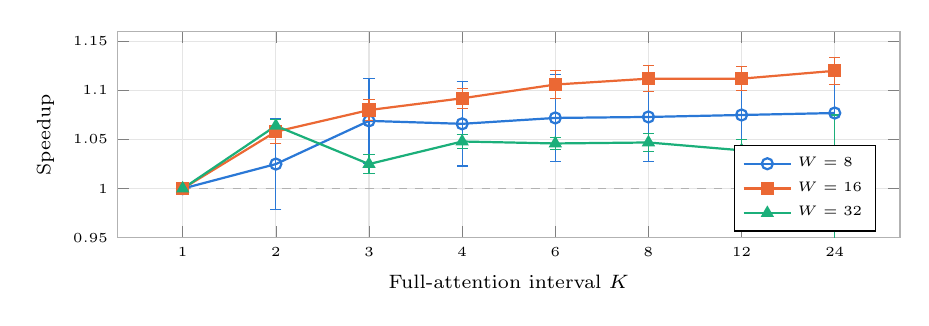
\begin{tikzpicture}
        \begin{axis}[
            width=0.95\columnwidth, height=4.2cm,
            xlabel={Full-attention interval $K$}, ylabel={Speedup},
            symbolic x coords={1,2,3,4,6,8,12,24},
            xtick=data,
            ymin=0.95, ymax=1.16,
            ytick={0.95,1.00,1.05,1.10,1.15},
            legend pos=south east, legend style={font=\tiny, cells={anchor=west}},
            grid=major, grid style={gray!20},
            axis line style={gray!60}, tick label style={font=\tiny}, label style={font=\scriptsize},
            error bars/y dir=both, error bars/y explicit,
        ]
            \addplot[seriesFull, mark=o, thick, mark options={fill=seriesFull}]
                coordinates {
                    (1,1.000)+-(0,0) (2,1.025)+-(0,0.046) (3,1.069)+-(0,0.043) (4,1.066)+-(0,0.043)
                    (6,1.072)+-(0,0.044) (8,1.073)+-(0,0.045) (12,1.075)+-(0,0.043) (24,1.077)+-(0,0.043)
                };
            \addlegendentry{$W=8$}
            \addplot[seriesWindowed, mark=square*, thick, mark options={fill=seriesWindowed}]
                coordinates {
                    (1,1.000)+-(0,0) (2,1.058)+-(0,0.012) (3,1.080)+-(0,0.011) (4,1.092)+-(0,0.010)
                    (6,1.106)+-(0,0.014) (8,1.112)+-(0,0.013) (12,1.112)+-(0,0.012) (24,1.120)+-(0,0.014)
                };
            \addlegendentry{$W=16$}
            \addplot[seriesAqua, mark=triangle*, thick, mark options={fill=seriesAqua}]
                coordinates {
                    (1,1.000)+-(0,0) (2,1.064)+-(0,0.006) (3,1.025)+-(0,0.010) (4,1.048)+-(0,0.007)
                    (6,1.046)+-(0,0.006) (8,1.047)+-(0,0.009) (12,1.039)+-(0,0.011) (24,1.008)+-(0,0.067)
                };
            \addlegendentry{$W=32$}
            \draw[gray!60, dashed] (axis cs:1,1.0) -- (axis cs:24,1.0);
        \end{axis}
    \end{tikzpicture}
    \caption{Window-sweep data (Table~\ref{tab:window-sweep}) with 95\% CIs. $W{=}16$ dominates at
    every $K$; $W{=}32$ degrades and grows noisy at high $K$; $W{=}8$ never catches up. $W{=}16$'s
    $K{=}24$ result and $W{=}8$'s have non-overlapping 95\% CIs -- a genuine effect of window size.}
    \label{fig:window-sweep-plot}
\end{figure}

\subsection{Quality validation}
\label{sec:quality-validation}
\emph{Distillation training and quality validation ran on a separate H200/CUDA machine, not the
target M5 Max.} We fine-tune only the windowed blocks' self-attention parameters by distillation
against the frozen teacher's own predictions, warm-started from pretrained weights. Training used
56 real teacher-generated images for 3000 steps (loss dropped $\sim$5$\times$). We validate on 8
held-out images at the decoded-mesh and decoded-Gaussian level, calibrating every divergence number
against the frozen teacher's own seed-to-seed variance (Table~\ref{tab:quality},
Figure~\ref{fig:quality-bars}) -- distinguishing genuine degradation from the sampler's inherent
stochastic sensitivity.

\begin{table}[t]
    \centering
    \caption{Distilled-student divergence, calibrated against seed-variance baseline. Below
    1.0$\times$: smaller than the teacher's own natural variation.}
    \label{tab:quality}
    \resizebox{\columnwidth}{!}{
    \begin{tabular}{@{}lrrr@{}}
        \toprule
        Channel & Baseline & Student & Ratio \\
        \midrule
        SLat feature (rel.\ error) & 0.337 & 0.440 & 1.31$\times$ \\
        Gaussian position (xyz) & 0.0133 & 0.0120 & \textbf{0.90$\times$} \\
        Gaussian color/SH & 0.286 & 0.316 & 1.11$\times$ \\
        Gaussian opacity & 0.136 & 0.150 & 1.10$\times$ \\
        Gaussian scale & 0.348 & 0.330 & \textbf{0.95$\times$} \\
        \bottomrule
    \end{tabular}}
\end{table}

\begin{figure}[t]
    \centering
    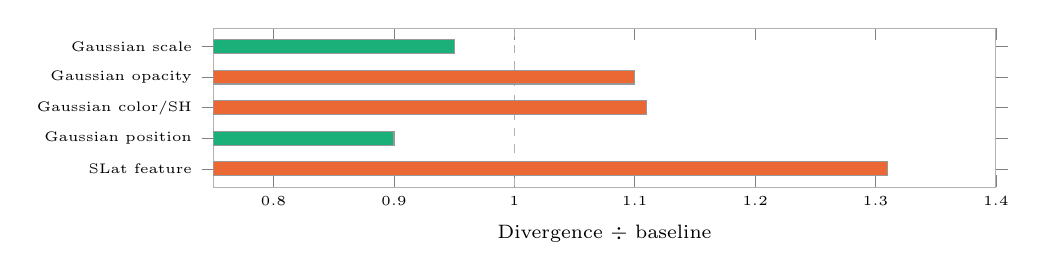
\begin{tikzpicture}
        \begin{axis}[
            width=0.95\columnwidth, height=3.6cm,
            xbar, bar width=5pt,
            xlabel={Divergence $\div$ baseline},
            xmin=0.75, xmax=1.4,
            xtick={0.8,0.9,1.0,1.1,1.2,1.3,1.4},
            symbolic y coords={Gaussian scale, Gaussian opacity, Gaussian color/SH, Gaussian position, SLat feature},
            ytick={Gaussian scale, Gaussian opacity, Gaussian color/SH, Gaussian position, SLat feature},
            y dir=reverse,
            axis line style={gray!60}, tick label style={font=\tiny}, label style={font=\scriptsize},
            enlarge y limits=0.15,
            extra x ticks={1.0},
            extra x tick labels={},
            extra tick style={grid=major, grid style={gray!60, dashed}, major tick length=0pt},
        ]
            \addplot[fill=seriesAqua, draw=black!40, bar shift=0pt] coordinates {(0.95,Gaussian scale)};
            \addplot[fill=seriesWindowed, draw=black!40, bar shift=0pt] coordinates {(1.10,Gaussian opacity)};
            \addplot[fill=seriesWindowed, draw=black!40, bar shift=0pt] coordinates {(1.11,Gaussian color/SH)};
            \addplot[fill=seriesAqua, draw=black!40, bar shift=0pt] coordinates {(0.90,Gaussian position)};
            \addplot[fill=seriesWindowed, draw=black!40, bar shift=0pt] coordinates {(1.31,SLat feature)};
        \end{axis}
    \end{tikzpicture}
    \caption{Table~\ref{tab:quality}'s five channels vs.\ the seed-variance baseline (dashed line
    at 1.0$\times$). Green: at/below baseline; orange: 10--31\% above.}
    \label{fig:quality-bars}
\end{figure}

Two of five channels (Gaussian position, scale) land at or below the natural seed-variance
baseline; the remaining three (SLat feature, color/SH, opacity) sit modestly above it
(1.10--1.31$\times$), a real but small excess attributable to the architecture change. An earlier
300-step checkpoint showed larger excess throughout (1.15--1.45$\times$); the consistent
improvement with more training suggests the gap is a function of training budget, though we have
not tested beyond 3000 steps. Mesh structure is essentially unchanged (vertex-count ratio 1.000,
Chamfer distance 0.0122 vs.\ 0.0125 at 300 steps).

\section{Discussion}

The central kernel-level finding is that hand-written \code{matmul2d} kernels, across every
configuration tested, do not reliably outperform \code{MPSGraph} on this hardware for this
workload's shape profile -- despite dedicated Neural Accelerator hardware and documentation
suggesting int8/precision-relaxation should help. Independent, concurrent work
(Rigel~\cite{rigel}) reverse-engineers the same \code{matmul2d}/MPP path at the microarchitectural
level on an M4 Max (the preceding, non-Neural-Accelerator generation), finding it runs on ordinary
shader cores with no dedicated matrix datapath and that fp8 is emulated, not accelerated -- a
different generation and method, but a consistent, independent, mechanism-level account of why
\code{matmul2d} does not reliably beat native \code{MPSGraph}. Confirming this directly on M5 Max
is future work. The framework baselines complicate the story further: MLX's non-MPP attention
kernel is $4.02\times$ faster than PyTorch at the identical hardware and shape, so the ceiling our
kernel work approached reflects PyTorch's MPS backend specifically, not a hardware ceiling; but
\code{llama.cpp}'s own non-MPP kernel does not replicate MLX's advantage, so something specific to
MLX's design (manual scalar dot products, \code{simd\_sum} reduction) -- not merely avoiding MPP --
is responsible. This advantage also has a real boundary, though not the one our own first
measurement suggested: at a short-sequence shape from a genuinely different model family
(ViT-L/14), MLX's advantage narrows sharply ($4.02\times \to 1.18\times$) rather than reversing --
our initial single-run result showed a reversal, which we caught only by replicating the
measurement 8 independent times and finding the opposite direction every time, and report as a
methodological lesson about measurement reliability at sub-millisecond scale rather than as a
finding about MLX itself. A same-shape cross-hardware check on an NVIDIA H200 finds no comparable
narrowing or instability in PyTorch's own CUDA backend-selection behavior, suggestive (not
confirmed, given only one cross-hardware data point) that both the narrowing and the instability
are specific to Apple Silicon/MLX rather than a universal short-sequence property. Identifying
precisely what about MLX's design produces both the long-sequence advantage and its short-sequence
narrowing is the highest-value open question this line of work raises.
\textbf{Practical takeaway for practitioners deploying attention-heavy models on Apple Silicon
today}: prefer MLX over PyTorch MPS for attention generally -- it remains faster at every shape we
tested, from a $4.02\times$ advantage at long sequences ($L$ in the thousands, as in TRELLIS or
Llama-class models) down to a smaller but still real $1.18\times$ at short, vision-transformer-style
sequences ($L$ in the low hundreds). At that short-sequence regime specifically, budget for
substantially more measurement noise than at longer sequences before trusting any single
benchmark's direction (Table~\ref{tab:vit}'s discussion above) -- our own first attempt at exactly
this measurement got the sign wrong.

The algorithmic-level results tell a different story: real speedups were available without
touching any kernel, by exploiting redundancy already present in the sampling procedure. This
suggests that for workloads of this shape, algorithmic optimization is currently more productive
than low-level kernel engineering on this hardware -- a conclusion reached only after exhausting
the kernel-level avenue with equal rigor. The architecture-level result sits between the two: it
changes what is computed, requiring a light fine-tune, and echoes the kernel-level pattern that an
implementation-quality gap, not an algorithmic ceiling, determined the outcome -- windowed
attention at the window size already trusted elsewhere in this codebase is \emph{slower} than full
attention in isolation, only becoming visible once the measurement was isolated and statistically
validated rather than trusted at the full-model level. Concurrent work on artist-quality mesh
retopology (TriFlow~\cite{triflow}) targets a problem distinct from but complementary to our own
dense mesh-decoder output -- whether a TriFlow-style post-process could improve our own output's
artist-usability is a real, untested question for future work.

\section{Limitations and Future Work}

All measurements ran on a single Apple M5 Max; whether these findings hold across M1--M4 hardware
(lacking the Neural Accelerator) is untested and the highest-leverage extension if pursued further.
Kernel- and algorithmic-level results are specific to TRELLIS's shape profile; we partially address
this via the framework comparison at substantially different shapes
(Section~\ref{sec:framework-baselines}), including a genuinely different model family
(ViT-L/14), but a full second model port remains untested. Most
kernel- and algorithmic-level timings are single-run wall-clock rather than repeated-trial with
confidence intervals -- the framework baselines and the architecture-level speed result are
exceptions ($n{=}8$/$n{=}20$, reported CIs) -- a real gap against top-tier-venue statistical rigor
for the remaining results. Both algorithmic results are verified on a convenience sample of six
(image, seed) combinations using voxel IoU and mesh-complexity proxies rather than an established
perceptual metric. The architecture-level quality validation used 56 training / 8 held-out images,
a single $(K, W, \text{budget})$ configuration, and ran on different hardware (H200/CUDA) from
every wall-clock measurement in this paper -- a practical necessity for affordable fine-tuning,
not expected to affect the architecture's hardware-independent training, but not independently
re-verified on the Apple Silicon target. Beyond repeating this hardware and model-generality sweep,
directly useful next steps include: identifying specifically what about MLX's kernel design
achieves its advantage over both PyTorch and \code{llama.cpp}; replacing our fixed-interval CFG
trigger with AB-Cache's fully adaptive, error-gated one; sweeping the full $(K,W,\text{budget})$
quality space rather than one configuration; and an appearance-level \emph{rendered} comparison,
currently blocked by the absence of a CUDA toolkit for compiling rendering extensions in our
distillation environment.

\section{Conclusion}

We presented a falsification-driven empirical study of Metal Performance Primitives on Apple
Silicon, using a real image-to-3D diffusion transformer as testbed. Hand-written \code{matmul2d}
kernels, refined across six operand-type combinations and three attention-kernel designs, closed
most but not all of the gap to PyTorch's native MPS backend, corroborated by an independent finding
that MLX avoids MPP for attention entirely -- a finding that replicates at a substantially
different long-sequence shape and narrows sharply, but does not reverse, at a short-sequence shape
from a genuinely different model family (ViT-L/14), after we caught and corrected our own first
measurement there, which showed a reversal that failed to replicate across 8 independent re-runs.
A cross-hardware check on an NVIDIA H200 finds no comparable narrowing or instability. Motivated by
this ceiling, we identified and fixed a
real algorithmic opportunity in TRELLIS's CFG sampler, delivering verified, generalizing speedups
without retraining. Finally, motivated by attention's dominant time-share, we explored an
architecture-level intervention -- interleaved full/windowed self-attention -- finding that window
size, not merely how many blocks are windowed, determines whether this helps or hurts at the
wall-clock level. After distillation, quality on held-out images is mixed but modest: two of five
channels are indistinguishable from natural seed-to-seed variation, the remaining three sit
10--31\% above it. We release all kernels, sampler code, architecture code, and measurement
scripts to support reproduction and extension of all three results.

\begin{thebibliography}{9}

\bibitem{trellis2024}
J.\ Xiang, Z.\ Lv, S.\ Xu, Y.\ Deng, R.\ Wang, B.\ Zhang, D.\ Chen, X.\ Tong, J.\ Yang.
\emph{Structured 3D Latents for Scalable and Versatile 3D Generation}.
arXiv:2412.01506, 2024.

\bibitem{flashattention}
T.\ Dao, D.\ Y.\ Fu, S.\ Ermon, A.\ Rudra, C.\ R\'{e}.
\emph{FlashAttention: Fast and Memory-Efficient Exact Attention with IO-Awareness}.
arXiv:2205.14135, 2022.

\bibitem{llmint8}
T.\ Dettmers, M.\ Lewis, Y.\ Belkada, L.\ Zettlemoyer.
\emph{LLM.int8(): 8-bit Matrix Multiplication for Transformers at Scale}.
arXiv:2208.07339, 2022.

\bibitem{swin}
Z.\ Liu, Y.\ Lin, Y.\ Cao, H.\ Hu, Y.\ Wei, Z.\ Zhang, S.\ Lin, B.\ Guo.
\emph{Swin Transformer: Hierarchical Vision Transformer using Shifted Windows}.
ICCV 2021, arXiv:2103.14030.

\bibitem{fastercache}
FasterCache: Training-Free Video Diffusion Model Acceleration with High Quality.
arXiv:2410.19355, 2024.

\bibitem{abcache}
AB-Cache: Adaptive Bias-Aware Caching for Accelerating Diffusion Models.
arXiv:2504.10540, 2025.

\bibitem{rigel}
R.\ Kumaresan.
\emph{Rigel: Reverse-Engineering the Metal 4.1 Tensor Compute Path on the Apple M4 Max GPU}.
arXiv:2606.12765, 2026.

\bibitem{mlx}
Apple.
\emph{MLX: An array framework for Apple Silicon}.
\url{https://github.com/ml-explore/mlx}, 2024.

\bibitem{ggml}
G.\ Gerganov et al.
\emph{llama.cpp: LLM inference in C/C++} (GGML tensor library and Metal backend).
\url{https://github.com/ggml-org/llama.cpp}, 2023.

\bibitem{triflow}
H.\ Li, Z.\ Erko\c{c}, D.\ Sirigatti, V.\ Rosov, L.\ Li, A.\ Dai, M.\ Nie\ss{}ner.
\emph{TriFlow: Generating Artist-Like 3D Mesh Topology via Nearest-Vertex Vector Fields}.
arXiv:2606.20131, 2026.

\end{thebibliography}

\appendix
\onecolumn
\section{Generalization at a different shape profile}
\label{app:generalization-shape}
\begin{table}[h]
    \centering
    \caption{Framework comparison at a substantially different (Llama-2-7B-like) shape profile,
    same protocol as Table~\ref{tab:frameworks}: $n{=}20$ trials, mean $\pm$ 95\% CI.}
    \begin{tabular}{@{}lrrr@{}}
        \toprule
        Operation & PyTorch MPS & MLX & \code{llama.cpp}/GGML \\
        \midrule
        Linear (2048$\times$4096$\to$4096) & 1.335ms $\pm$ 0.025 & 1.333ms $\pm$ 0.011 & 1.633ms $\pm$ 0.064 \\
        Self-attention ($H{=}32$, $L{=}2048$, $D{=}128$) & 5.183ms $\pm$ 0.023 & \textbf{1.600ms $\pm$ 0.017} & 6.056ms $\pm$ 0.039 \\
        \bottomrule
    \end{tabular}
\end{table}

\section{Generalization across images and seeds}
\label{app:generalization-images}
\begin{table}[h]
    \centering
    \caption{Generalization across three additional example images and two seeds each.}
    \begin{tabular}{@{}llrrrr@{}}
        \toprule
        Image & Seed & 8-step speedup & 8-step IoU & CFG-diff(4) speedup & CFG-diff(4) IoU \\
        \midrule
        vase & 1 & 1.75$\times$ & 0.7773 & 1.13$\times$ & 0.7494 \\
        vase & 2 & 1.92$\times$ & 0.9512 & 1.16$\times$ & 0.8332 \\
        dragon & 1 & 1.99$\times$ & 0.8657 & 1.27$\times$ & 0.8289 \\
        dragon & 2 & 1.91$\times$ & 0.8161 & 1.18$\times$ & 0.7726 \\
        biplane & 1 & 2.14$\times$ & 0.9369 & 1.30$\times$ & 0.8874 \\
        biplane & 2 & 2.17$\times$ & 0.9282 & 1.25$\times$ & 0.8173 \\
        \midrule
        \textbf{Average} & & \textbf{1.98$\times$} & \textbf{0.8792} & \textbf{1.22$\times$} & \textbf{0.8148} \\
        \bottomrule
    \end{tabular}
\end{table}

\section{Interleaved attention: connectivity schematic}
\label{app:arch-diagram}
\begin{figure}[h]
    \centering
    \begin{subfigure}[b]{0.48\textwidth}
        \centering
        
\begin{tikzpicture}[scale=0.85, tok/.style={circle, fill=seriesFull, draw=black!50, minimum size=5mm, inner sep=0}]
            \foreach \i in {0,...,7} {
                \node[tok] (t\i) at ({90 - \i*45}:1.3) {};
            }
            \foreach \i in {0,...,7} {
                \foreach \j in {0,...,7} {
                    \ifnum\i<\j
                        \draw[seriesFull!70, line width=0.35pt] (t\i) -- (t\j);
                    \fi
                }
            }
        \end{tikzpicture}
        \caption{Full attention: every token attends to every other -- $O(N^2)$ edges.}
    \end{subfigure}
    \hfill
    \begin{subfigure}[b]{0.48\textwidth}
        \centering
        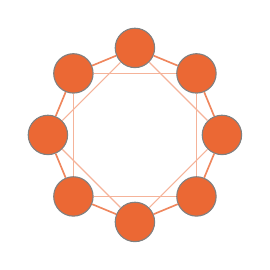
\begin{tikzpicture}[scale=0.85, tok/.style={circle, fill=seriesWindowed, draw=black!50, minimum size=5mm, inner sep=0}]
            \foreach \i in {0,...,7} {
                \node[tok] (t\i) at ({90 - \i*45}:1.3) {};
            }
            \foreach \i in {0,...,7} {
                \pgfmathtruncatemacro{\jone}{mod(\i+1,8)}
                \pgfmathtruncatemacro{\jtwo}{mod(\i+2,8)}
                \draw[seriesWindowed!80, line width=0.6pt] (t\i) -- (t\jone);
                \draw[seriesWindowed!50, line width=0.4pt] (t\i) -- (t\jtwo);
            }
        \end{tikzpicture}
        \caption{Windowed attention: local neighborhood only -- $O(N{\cdot}W)$ edges, $W{\ll}N$.}
    \end{subfigure}
    \caption{Connectivity schematic underlying Figure~\ref{fig:block-strip}'s block assignment.}
\end{figure}

\end{document}
